Per \textit{servizio di visualizzazione di carte geografiche} si intende un sistema, disponibile in rete, che permette l'utilizzo e la consultazione di mappe geografiche. Nel corso di questo capitolo verrà illustrato il funzionamento e le caratteristiche principali dei maggiori competitor del settore.

\section{OpenStreetMap}

\textbf{OpenStreetMap (OSM)} è molto più di un semplice servizio di visualizzazione di mappe, volendo citare proprio la comunità che ha creato e gestisce il progetto: "OpenStreetMap is a map of the world, created by people like you and free to use under an open license" (\textit{OpenStreetMap è una mappa del mondo, creata da persone come te e utilizzata sotto licenza libera}).\cite{OSM}


\textit{OSM}, come si può capire dalla citazione, è un progetto sviluppato e realizzato da una comunità di persone. Fondato nel 2004 da Steve Coast con lo scopo di creare una mappa libera del mondo, nel 2006 ebbe inizio il processo per la trasformazione della società in fondazione non a scopo di lucro, da cui anche la rinominazione in \textbf{OpenStreetMaps Foundation}.

La \textit{"mappa"} negli anni ha subito diverse modifiche e soprattutto è cresciuta grazie alle donazioni non solo di utenti privati, ma sopratutto di enti e aziende quali ad esempio \textit{Automotive Navigation Data}, che nel 2007 donò il database stradale completo dei Paesi Bassi e quello delle principali strade di India e Cina.

La particolarità e l'unicità di questo progetto è sicuramente la sua licenza. Il database è pubblicato secondo la \textit{Open Database License}, la licenza che permette di condividere e adattare il database e creare opere a partire dallo stesso. Le uniche condizioni da rispettare secondo la \textit{ODbL} sono:
\begin{itemize}
\item attribuire l'appartenenza del database ad ogni suo utilizzo e ad ogni utilizzo di una banca dati derivata;
\item se viene pubblicato il database con una modifica rispetto all'originale o si creano nuovi database a partire da esso è obbligatorio distribuire il nuovo database secondo la licenza \textit{OBdL};
\item anche se il database venisse redistribuito in una nuova versione che ne restringa la libertà d'utilizzo, deve rimanere disponibile una versione aperta del database priva delle restrizioni.
\end{itemize}

Allo stesso modo del database, anche i dati inseriti e caricati dagli utenti devono rispettare una licenza compatibile con la Creative Commons e gli stessi contributori devono essere registrati al progetto.

Le modifiche operate sulla mappa vengono registrate in un elenco visibile sul sito web della fondazione, come visibile nella figura \ref{fig:OSMchangesets}.

I dati di \textit{OpenStreetMap} sono utilizzati inoltre da uno dei principali provider di questo settore, ovvero \textbf{Mapbox}. L'utilizzo di quest'ultimo lo abbiamo inconsciamente visto diverse volte navigando su internet, su siti web come \textit{Foursquare}, \textit{Pinterest}, \textit{Evernote}, \textit{Financial Times} e \textit{National Geographic}.\cite{mapbox:showcase}

\begin{figure}[H]
	\centering
		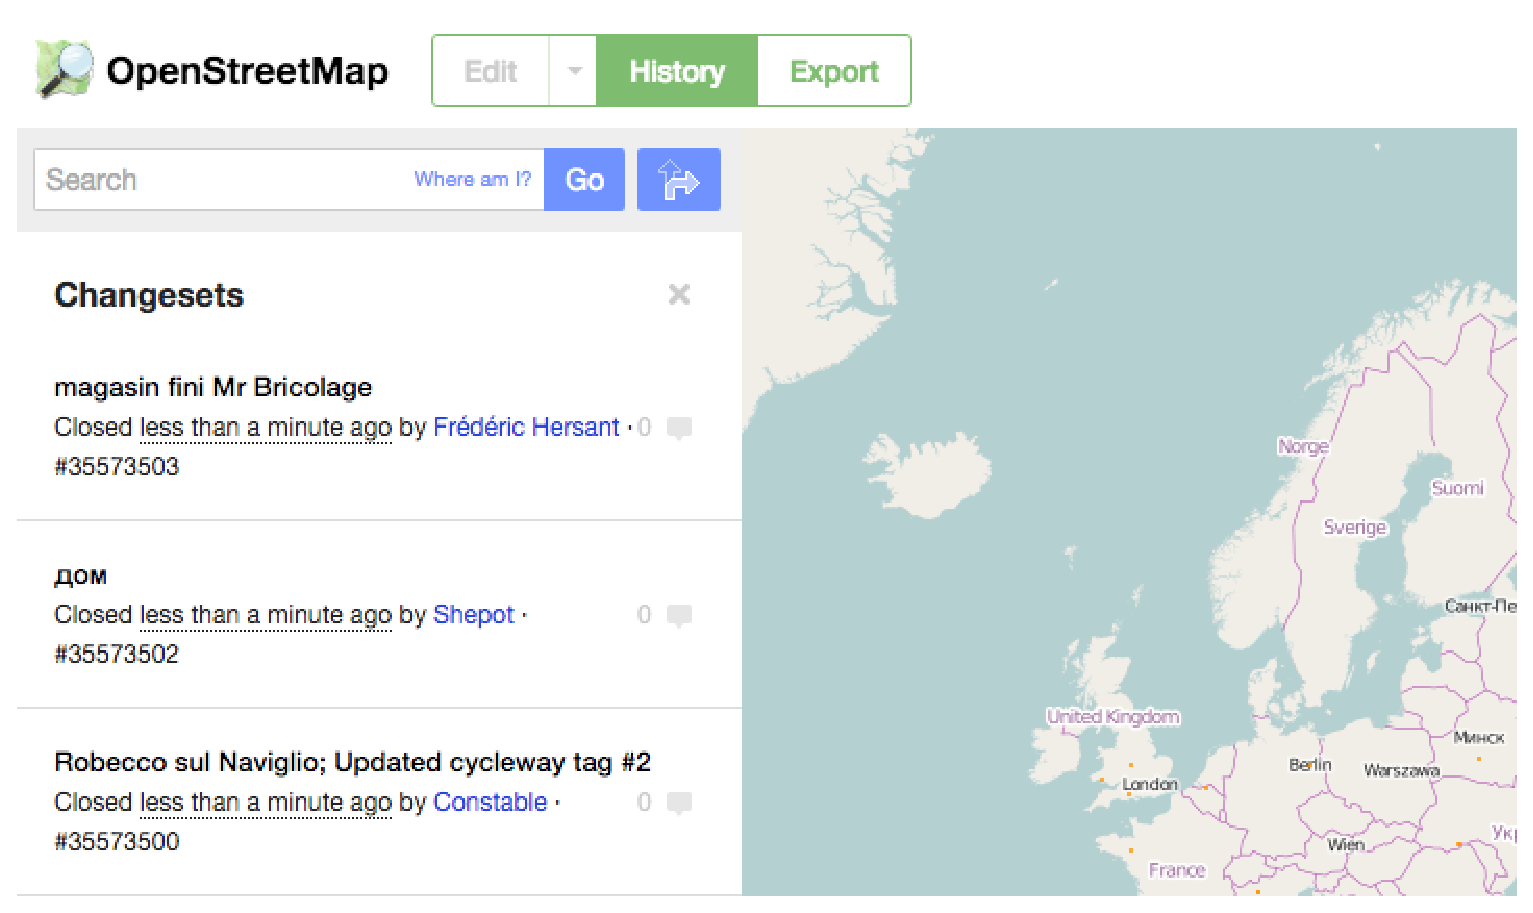
\includegraphics[scale=0.5]{figure/OSMchangesets.eps}
	\caption{Records di modifica della mappa ad opera di utenti} \label{fig:OSMchangesets}
\end{figure}

\section{Bing Maps}

Dopo aver visto un servizio \textit{open source}\footnote{Open Source\cite{wiki:opensource}} come \textit{OSM}, è importante vedere anche il competitor forse più \textit{"demonizzato"} dal mondo delle licenze libere. Infatti in questa sezione, descriveremo il funzionamento e le caratteristiche di \textbf{Bing Maps}, il sistema di \textit{web mapping}\footnote{Con "Web Mapping" si intende il processo di utilizzo o offerta di mappe sul World Wide Web} creato e sviluppato dalla Microsoft.

In questo servizio a differenza di \textit{OpenStreetMap} le mappe non sono curate da una comunità di developer ma raccolte ed elaborate in diversi modi. Anche Bing Maps come \textit{Mapbox} attinge ai database di OSM per le mappe stradali, che rappresentano la visualizzazione di default, ovvero la mappa che possiamo vedere appena accediamo alla pagina web del portale di Microsoft. È necessario però sottolineare, che a differenza dei due servizi sopra citati - OSM e Mapbox -, quello di Microsoft offre altre possibilità di visualizzazione delle cartine, consentendone anche una vista aerea, una cosiddetta "\textit{bird's-eye view}" (vista a volo d'uccello, che ne permette una visualizzazione prospettica di terreni e edifici), una veduta stradale che consente di vedere la strada a 360 gradi e infine troviamo la possibilità di accedere a mappe 3D in cui a prendere forma, oltre ai terreni e alle montagne, ci sono anche palazzi e monumenti. Di seguito vengono illustrati alcuni esempi di visualizzazione delle mappe di Bing:
\begin{figure}[ht]
	\centering
	\subfloat{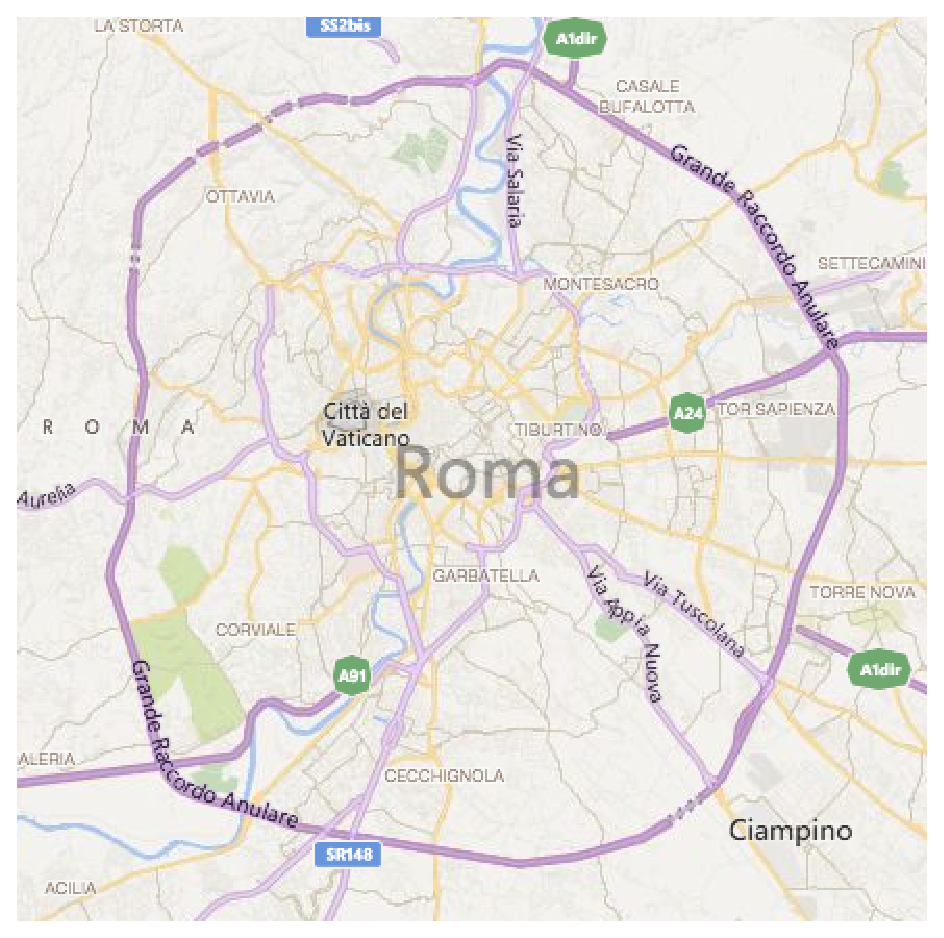
\includegraphics[scale=0.4]{figure/BINGRoadmap.eps}}
	\subfloat{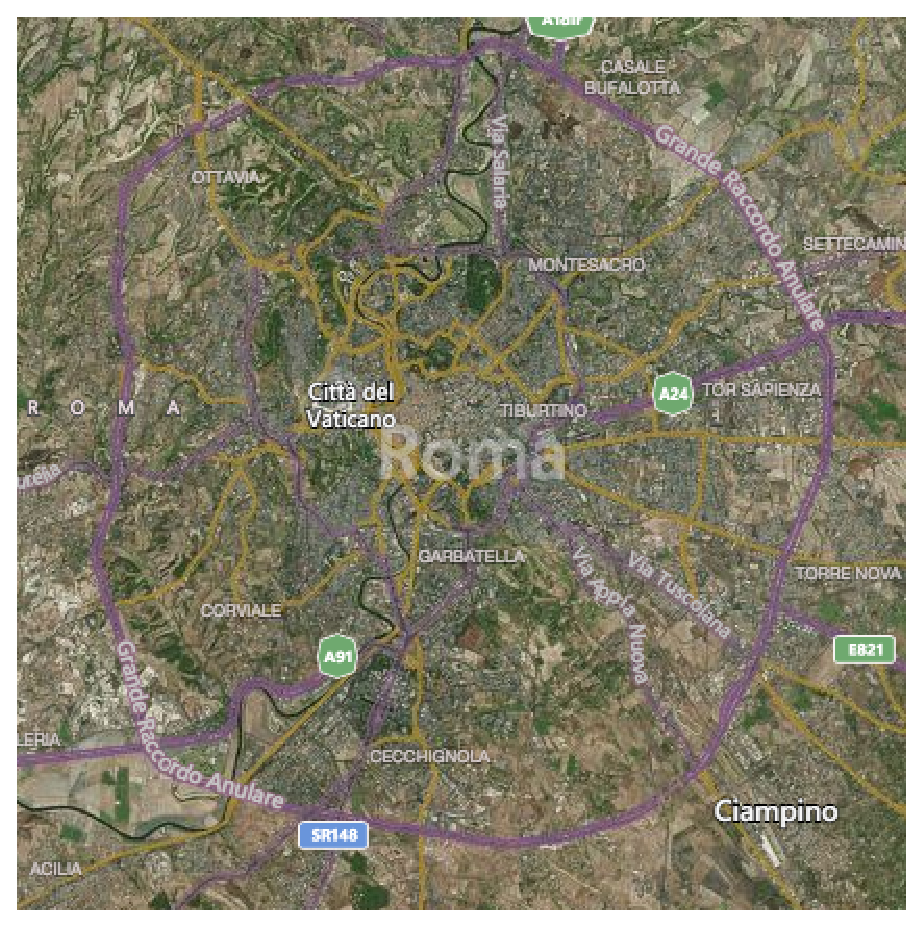
\includegraphics[scale=0.4]{figure/BINGAerial.eps}}
	\caption{Esempi di mappa stradale (a sinistra) e mappa aerea (a destra)}
\end{figure}

\begin{figure}[H]
	\centering
	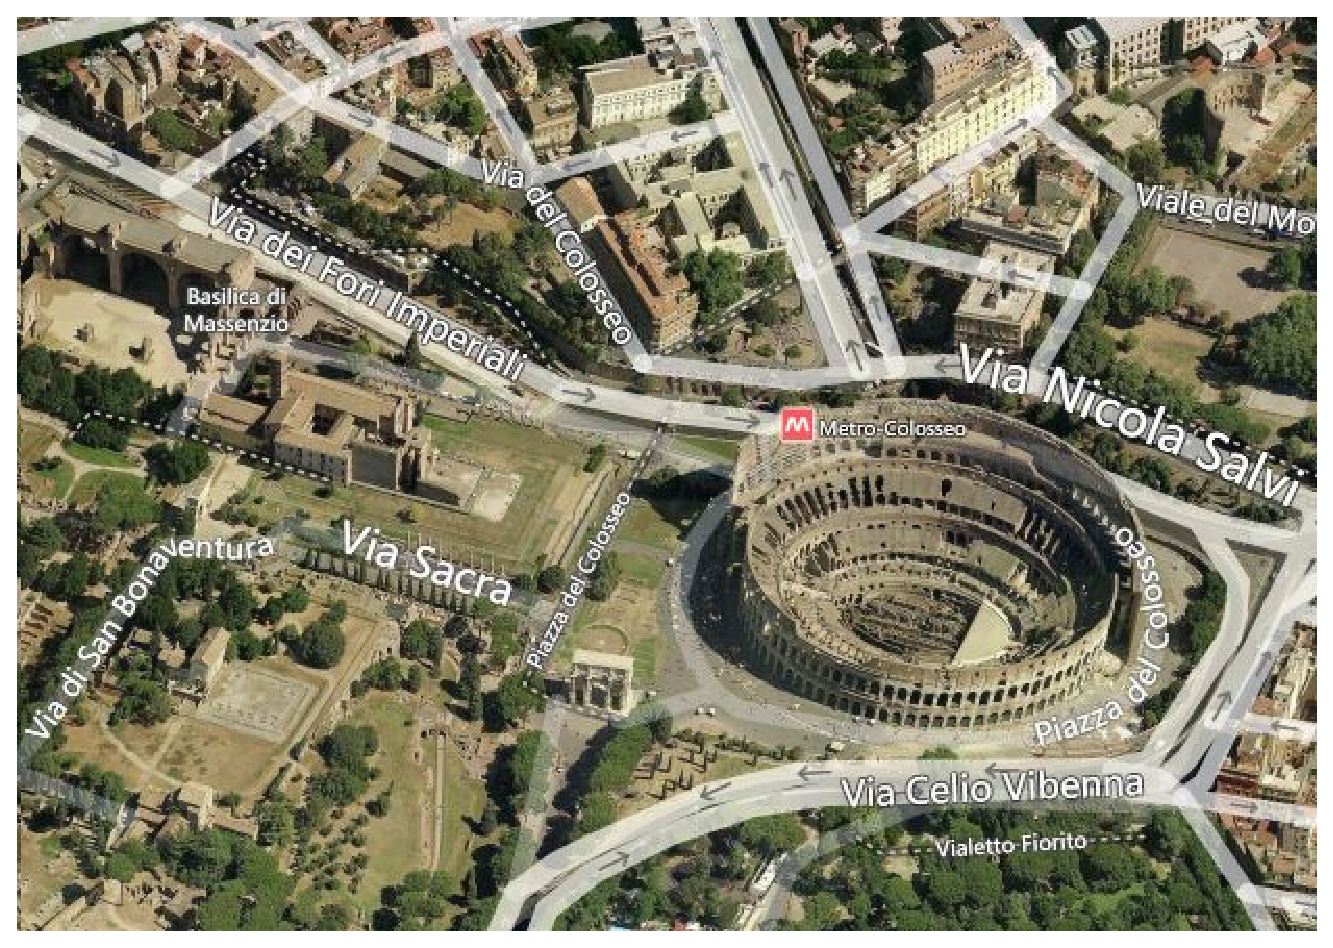
\includegraphics[scale=0.5]{figure/BINGBirdseye.eps}
	\caption{Esempio di visualizzazione Bird's-eye}
\end{figure}

Una delle peculiarità probabilmente più interessanti di Bing Maps, comunque, è la presenza al suo interno di differenti "Map Apps" delle vere e proprie applicazioni interne al servizio che ne sfruttano funzionalità e informazioni e ne arricchiscono così anche l'esperienza d'uso da parte dell'utente finale. Per fornire un esempio di questo utilizzo, si può far riferimento all'edizione del 2010 del \textit{Tour de France} che utilizzava la mappa Bing per mostrare risultati e tracciati delle differenti tappe della nota competizione ciclistica.\cite{bing:tdf}

\section{Google Maps}

Dopo aver trattato di \textit{OpenStreetMap} e \textit{Bing Maps}, era inevitabile parlare di quello che è, molto probabilmente, il sistema di visualizzazione cartografico più utilizzato nel mondo. Infatti in questo paragrafo, verrà descritto e analizzato \textit{Google Maps}, che è il servizio di mappe offerto e creato da \textit{Google Inc.}. Nato e reso disponibile nel 2005, a differenza dei due precedenti servizi non era stato ideato e pensato come servizio online, ma doveva essere un programma scritto in \textit{C++}\footnote{Il C++ è un linguaggio di programmazione orientato agli oggetti\cite{wiki:cpp}} e ideato dal cofondatore di \textit{Google} Lars Rasmussen e suo fratello Jens Eilstrup Rasmussen, successivamente il progetto venne convertito e rilasciato online come tutt'oggi lo conosciamo.

Le funzionalità di visualizzazione sono molto simili ai due servizi prima descritti. Infatti anche \textit{Google Maps} come \textit{Bing Maps}, offre agli utenti la possibilità di utilizzare e consultare mappe con vista satellitare, stradale o ibrida\footnote{La visualizzazioen ibrida permette all'utente di vedere il terreno con vista satellitare avendo anche il dettaglio delle strade}. Negli anni \textit{Google Maps} ha esteso molto le sue funzionalità e le sue caratteristiche. Nel tempo, infatti la società di Mountain View\footnote{La sede principale di \textit{Google Inc.} si trova a Mountain View in California} ha unito molti dei suoi progetti o prodotto \textit{ad hoc} servizi aggiuntivi, per aggiungerli al proprio servizio di mappe. Di seguito verranno elencati i principali servizi aggiuntivi offerti da \textit{Google Maps}:

\begin{itemize}
	\item\textbf{Google Traffic}: è un servizio disponibile in oltre di 50 paesi, che permette all'utente di conoscere la situazione del traffico in tempo reale;
	\item\textbf{Google Transit}: è il sistema che permette all'utente la pianificazione di un itinerario utilizzando esclusivamente i mezzi pubblici partito nel 2007, ad oggi serve centinaia di città in tutto il mondo;
	\item\textbf{Google Places}: attraverso questo servizio si può segnare sulla mappa una qualsiasi attività presente sul territorio (negozi, ristoranti, studi, ambulatori). I luoghi segnalati, verranno memorizzati e sarà disponibile una scheda dell'attività sotto la barra di ricerca ogin volta che selezioneremo il luogo sulla mappa;
	\item\textbf{Google Street View}: è probabilmente la caratteristica più conosciuta del sistema Maps. Il suo funzionamento permette di poter percorrere le strade di numerose città in tutto il mondo, immedesimandosi nella macchina di google che periodicamente percorre le strade per aggiornare le immagini.
\end{itemize}
Ho introdotto questo sistema di visualizzazione descrivendo come fosse, probabilmente, il più utilizzato in tutto il mondo. È importante, infatti, citare alcune delle applicazioni o società che utilizzano le API\footnote{Application Programming Interface\cite{wiki:api}} di \textit{Google Maps}. Infatti tra di esse spiccano i nomi di \textit{Whatsapp}, \textit{Airbnb}, \textit{Runtastic} o il \textit{New York Times}\cite{gmaps:show}

Entriamo, dunque, nel mezzo del mio progetto, perchè per realizzare il mio sistema di visualizzazione di mappe ho utilizzato proprio le API fornite da \textit{Google}, che avrò modo di illustrare maggiormente nel capitolo successivo.

\begin{figure}[ht]
	\centering
	\includegraphics[scale=0.5]{figure/googletraffic}
	\caption{Applicazione di Google Traffic sulla mappa di Roma}\label{fig:googletraffic}
\end{figure}